\chapter{Related work}
\label{ch:related}
This chapter discusses relevant related work that serves as inspiration for the work of this thesis. In Section~\ref{rw:multi-tenancy}, two different approaches for achieving multi-tenancy on top of Kubernetes including the consequences of tenant aggregation are discussed. The remaining sections discuss several existing state-of-art approaches related to the SLA-decomposition problem tackled in this thesis.  Section~\ref{rw:conclusion} argues which approach will be the basis of the work presented by this thesis. 
\section{Multi-tenancy via container orchestration}
\label{rw:multi-tenancy}
In the following sections discuss proposals made by members of both the Kubernetes working group and research community to adapt or leverage Kubernetes concepts to achieve multi-tenancy at different levels. 
\subsection{Hard multi-tenancy in Kubernetes: K8 is the new kernel}
Kubernetes, initially released in June 2014, is still under rapid development. Enabling support for multi-tenancy is one of the aspects the community's working group is focusing on. This section discusses some recent architectural proposals of the community to achieve hard multi-tenancy in Kubernetes. Information in this section is retrieved from a blog post~\footnote{\url{https://blog.jessfraz.com/post/hard-multi-tenancy-in-kubernetes/}} of Jessie Frazelle (\textit{Microsoft})~\cite{hardmultiproposals}, a respected former docker employee and Kubernetes working group member, and documents~\cite{hardmulti} of the K8's multi-tenancy working group. 

\subsubsection{Hard multi-tenancy}
Multi-tenancy, as discussed before, can be achieved on multiple levels in the technology stack. All focusing primarily on the improvement of resource utilization. Another differentiation, based on trust assumption between the tenants, can be made between to classify approaches. When tenants of a K8 cluster are assumed to be non-malicious and security isolation measures merely serve to prevent accidents, the term \textit{soft multi-tenancy} is used. Such as cluster sharing within one organization. Soft isolation often allows tenants to use unused resources that were allocated to other tenants, but enforce quotas when necessary~\cite{mozafari2013dbseer}. On the other hand, \textit{hard multi-tenancy} refers to the sharing of cluster resources among (potentially malicious) tenants from multiple organizations which do not fully trust each other. The remainder of the section focuses on achieving hard multi-tenancy in Kubernetes~\cite{hardmulti}.
\\\\
From a security point of view, Kubernetes has two potential attack surfaces:  unauthorized use of Kubernetes API and remote code execution in containers of running services. Different tenants should thus not be able to manipulate each other's clusters and their containers should be isolated. An exploit leading to supervisor privileges for a single tenant could have a devastating result.~\cite{hardmultiproposals} 

\subsubsection{Proposals}
For effective security, a system should be composed out of multiple layers. The failure of a single layer should not compromise the entire system. The following paragraphs discuss how such a multi-layered approach can be achieved within Kubernetes via the proposals of~\cite{hardmultiproposals}.

\begin{figure}
\centering
\subfigure[Namespaces on separate nodes.]{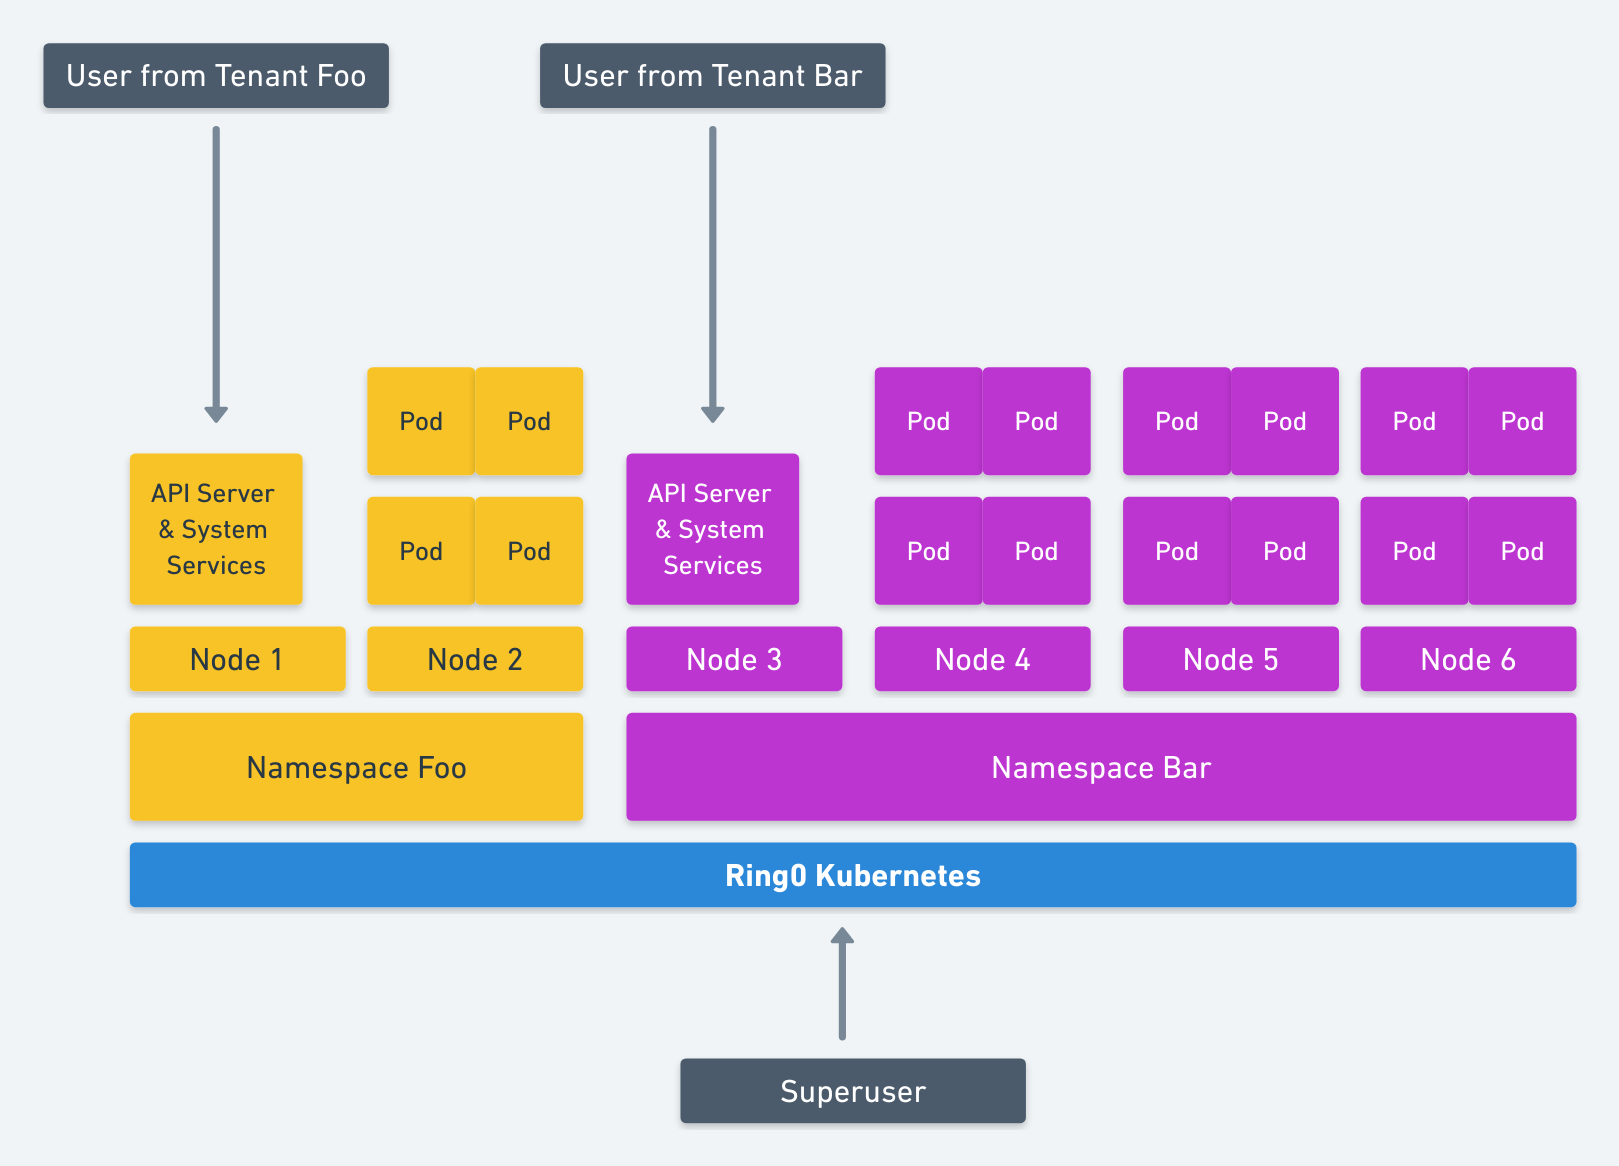
\includegraphics[width=0.7\linewidth]{chapter-related-work/images-hard/hard-multi-1.png}\label{fig:sub1}}
\subfigure[Namespace system services on shared node.]{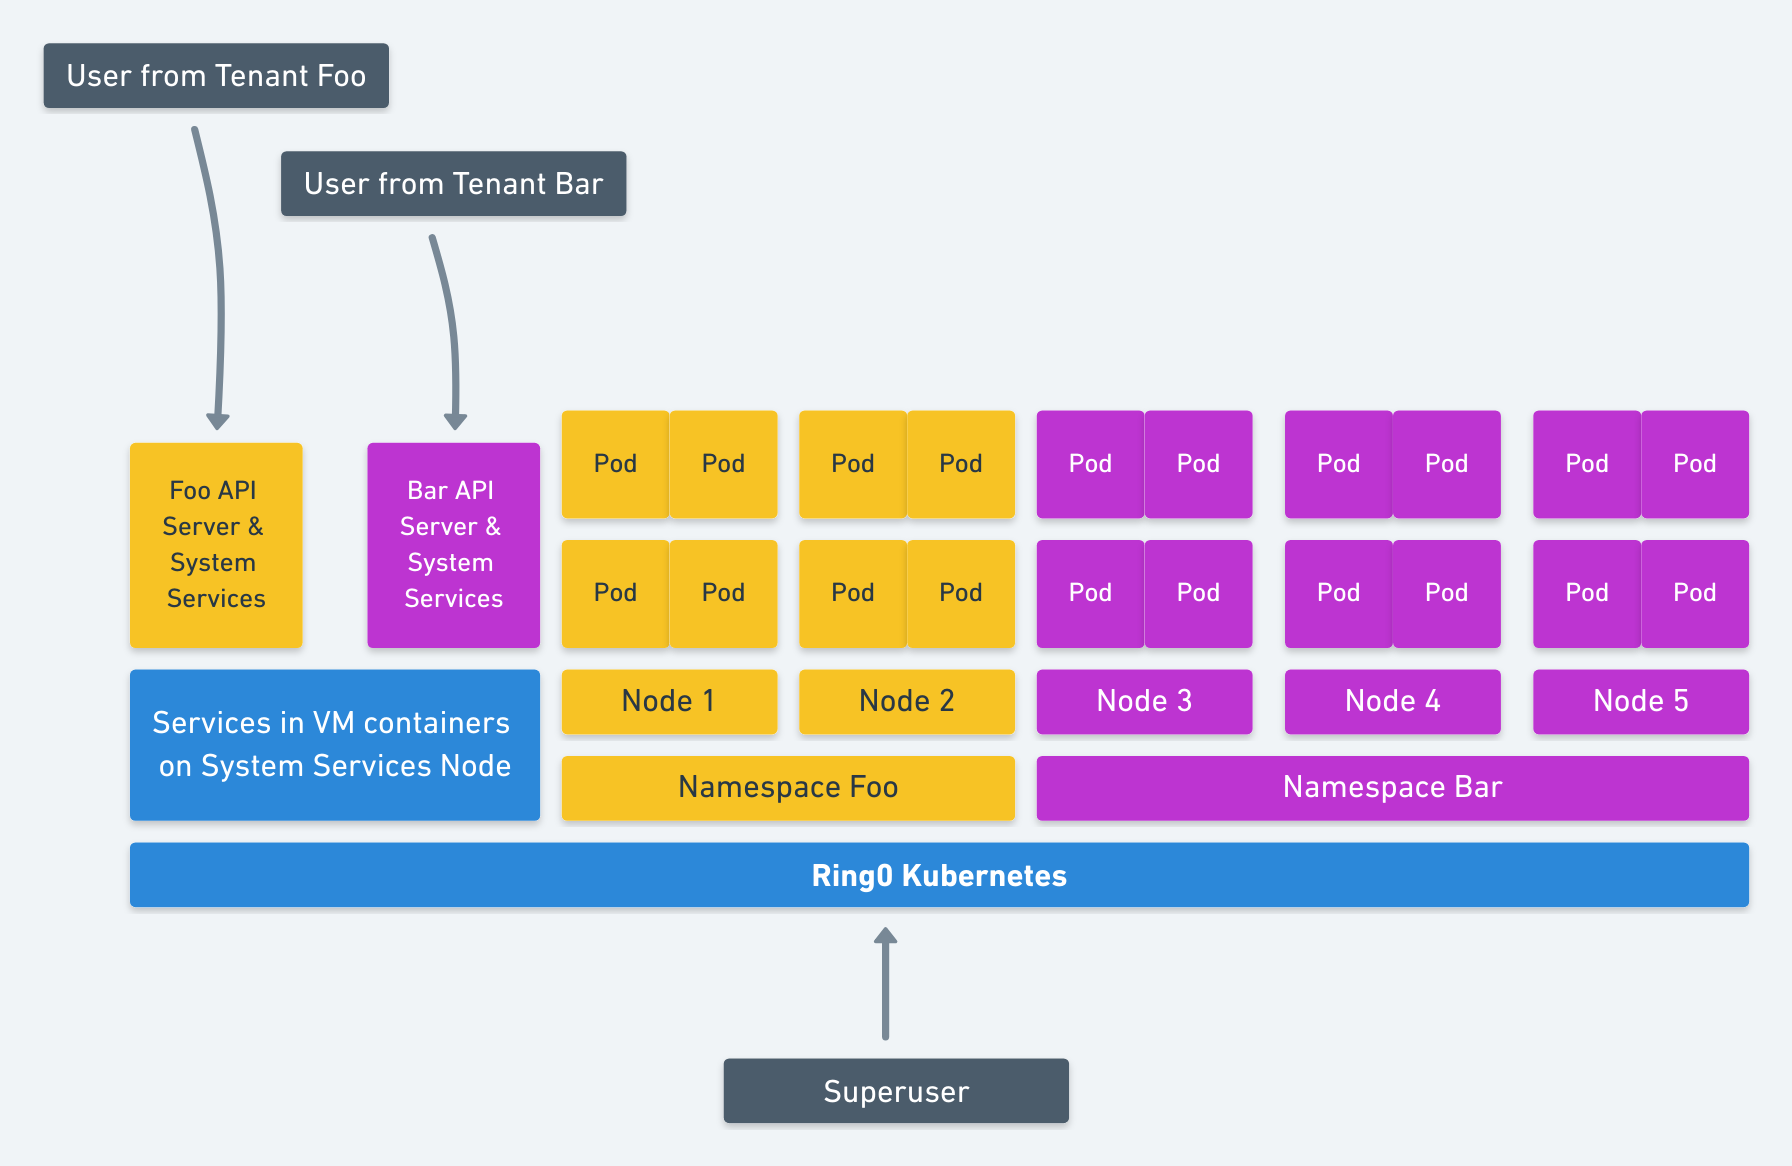
\includegraphics[width=0.7\linewidth]{chapter-related-work/images-hard/hard-multi-2.png}\label{fig:sub2}}
\subfigure[Containerized nodes to share physical nodes.]{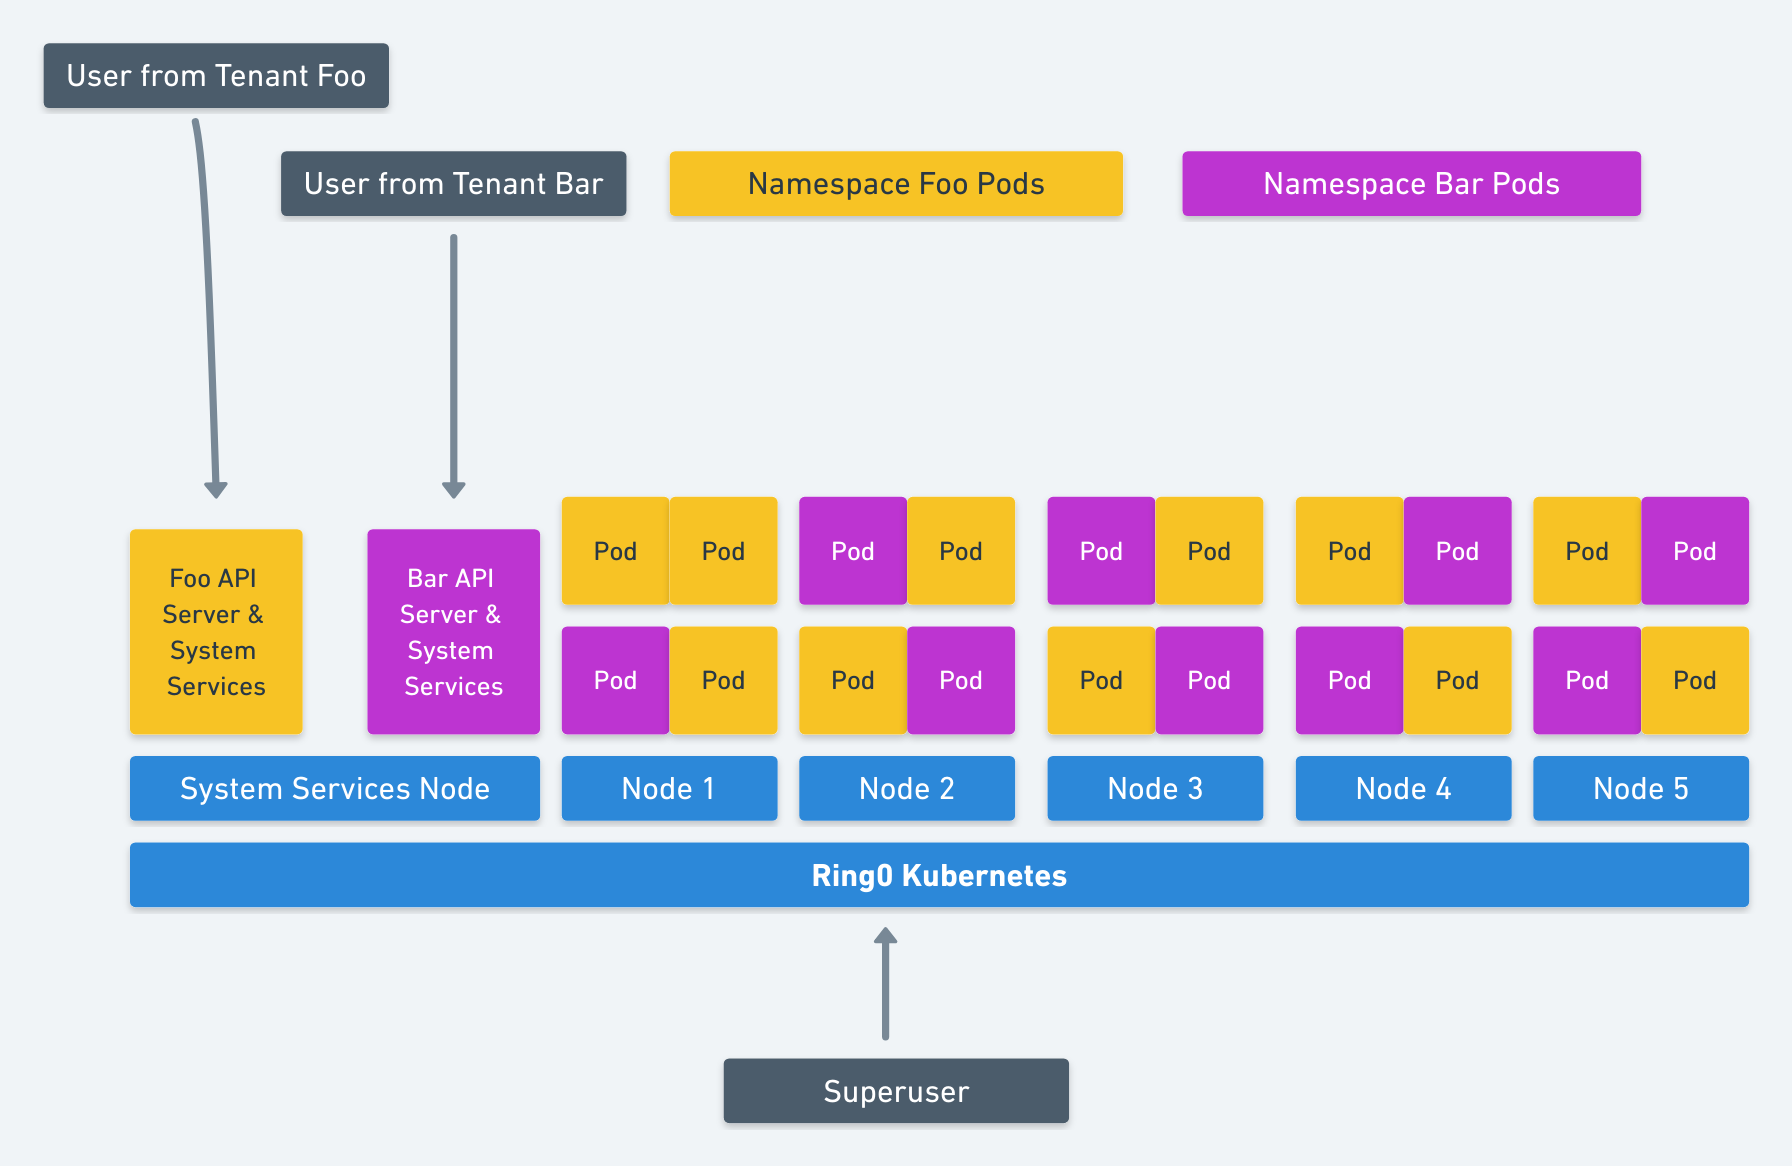
\includegraphics[width=0.7\linewidth]{chapter-related-work/images-hard/hard-multi-3.png}\label{fig:sub3}}
\caption{Proposal architecture for hard multi-tenancy in Kubernetes.~\cite{hardmultiproposals}}
\label{fig:hardmultiproposals}
\end{figure}

\paragraph{K8 in K8 Namespaces}
Kubernetes Namespaces are seen as a boundary for separating multiple users in the cluster. Kubernetes system services such as the API-server, however, are shared between these users. An exploit of a single namespace could possibly affect all the other namespaces. A proposal to eliminate this attack surface, is for each namespace to have its own Kubernetes system services (running in pods within that namespace). An exploit of these services would not grant access to the root Kubernetes services but be contained to the namespace. This idea borrows from Nested Kernel: Intra-Kernel Privilege Separation~\cite{dautenhahn2015nested}. Here, a small kernel nested inside the monolithic kernel allows for privilege isolation. By employing this nested structure,  users can strictly see the resources assigned to them in the namespace via their own system services. This matches the purpose of namespaces in Linux: what a process can see, is controlled by the namespace.~\cite{hardmultiproposals}

\paragraph{Nodes assigned to Namespaces}
Kubernetes namespaces currently employ quota (CPU and memory) to limit resources utilization of the services designated to them. In order to have even stricter isolation between services of different namespaces, a proposal is  a stricter assignment of what is exactly controlled by namespaces.
One possibility is to assign nodes at the machine level to a particular namespace. All services (including system services) would be constrainted to run on these machines. Services of different tenants would never run on the same machine. And namespaces would have no notion of other nodes. This strict assignment combined with the separate API from the previous paragraph is illustrated in Figure~\ref{fig:sub1}.~\cite{hardmultiproposals}\\\\
In order to achieve a better resource utilization, Kubernetes system services could be run in isolated VM containers (such as the Kata lightweight VM containers~\cite{katacontainers}) on a designated services node. This is shown in Figure~\ref{fig:sub2}.~\cite{hardmultiproposals}\\
A third option is to  completely virtualize the system. Here a node assigned to a namespace and on which containers are executed is itself a VM container. This enables the sharing of physical nodes between namespaces.  Figure~\ref{fig:sub3} illustrates this option.~\cite{hardmultiproposals}

\begin{figure}[H]
    \centering
    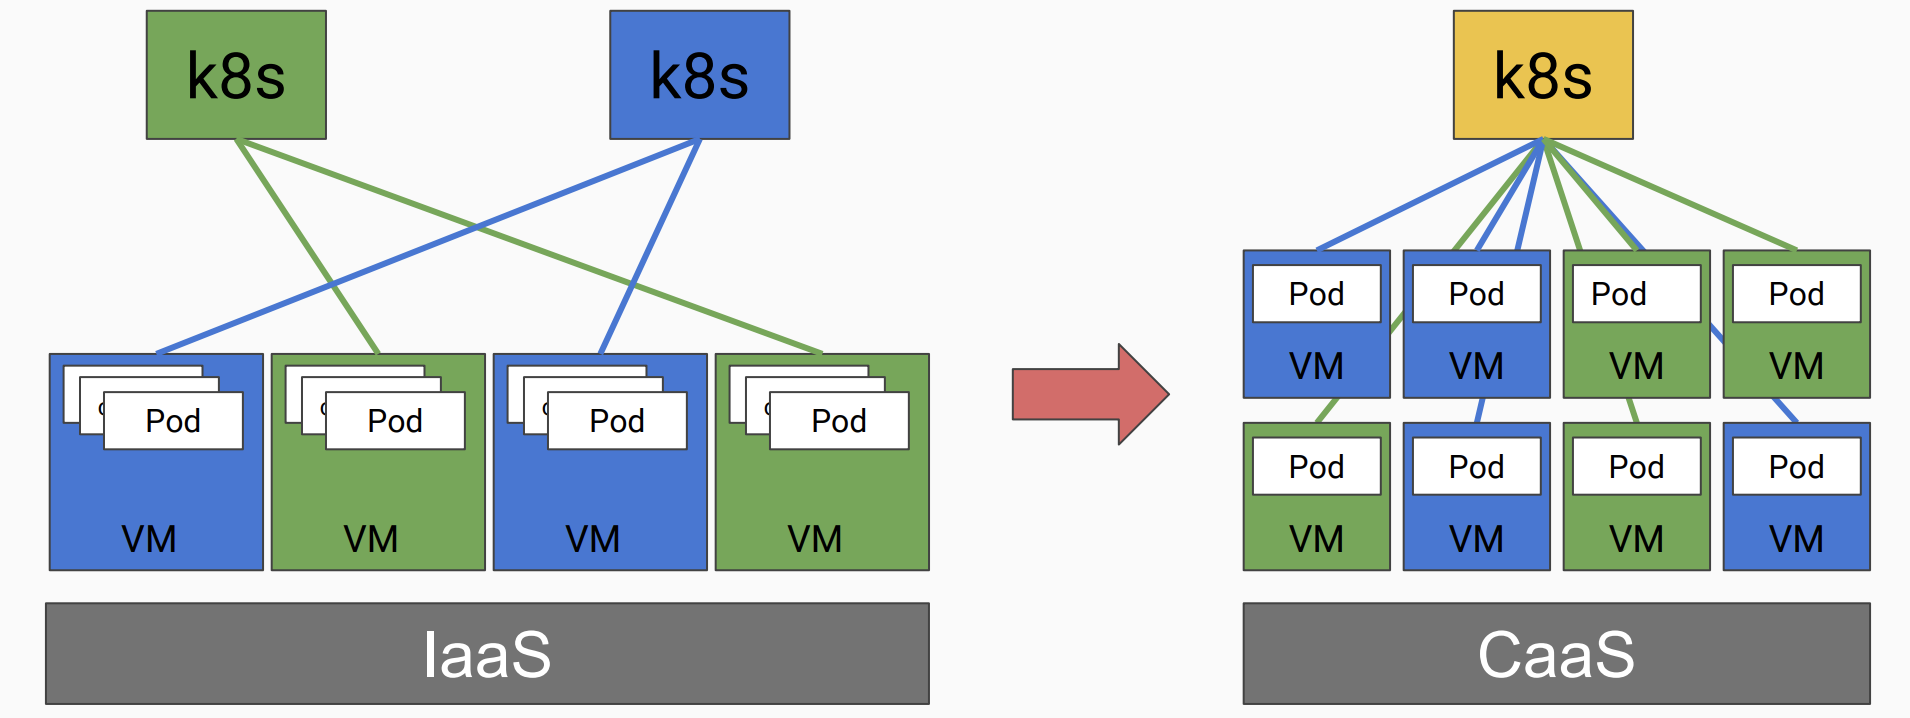
\includegraphics[width=0.9\textwidth]{chapter-related-work/images-hard/IaaS-to-CaaS.png}
    \caption{Evolution from IaaS to CaaS using containerized lightweight virtual machines.~\cite{kubernetes-deep-dive}}
    \label{fig:evolution}
\end{figure}

\subsubsection{Retrospect}
The proposals presented above diminish the attack surface for logical vulnerabilities of Kubernetes and the Kubernetes API by assigning each namespace its own separate system services. Additionally, containers from different namespaces are isolated by full virtualization. This is achieved by dedicated nodes or by containers running lightweight VMs. Combined these techniques deliver a strong solution for the threat model of hard multi-tenancy.\\\\
From a critical viewpoint, the question of the benefits of this model compared to running multiple separate Kubernetes clusters comes to mind. In the latter, resource sharing between clusters on a physical node happens at the level of virtual machines, which may be less efficient. An added benefit of the approach above is the less cumbersome administration of the cluster through its centralized nature. In essence, these approaches resemble the transition from Infrastructure as a service (Iaas) to Containers as a service (CaaS).
\newpage
\subsection{Towards a container-based architecture for multi-tenant SaaS applications.}
\label{rw:eddy}
The paper "\textit{Towards a container-based architecture for multi-tenant SaaS applications}"~\cite{TruyenEddy2016Taca} presents a container based middleware platform architecture and three possible deployment strategies to achieve multi-tenancy SaaS applications within a container orchestration environment. This work is briefly discussed in following paragraphs.
\begin{figure}[H]
    \centering
    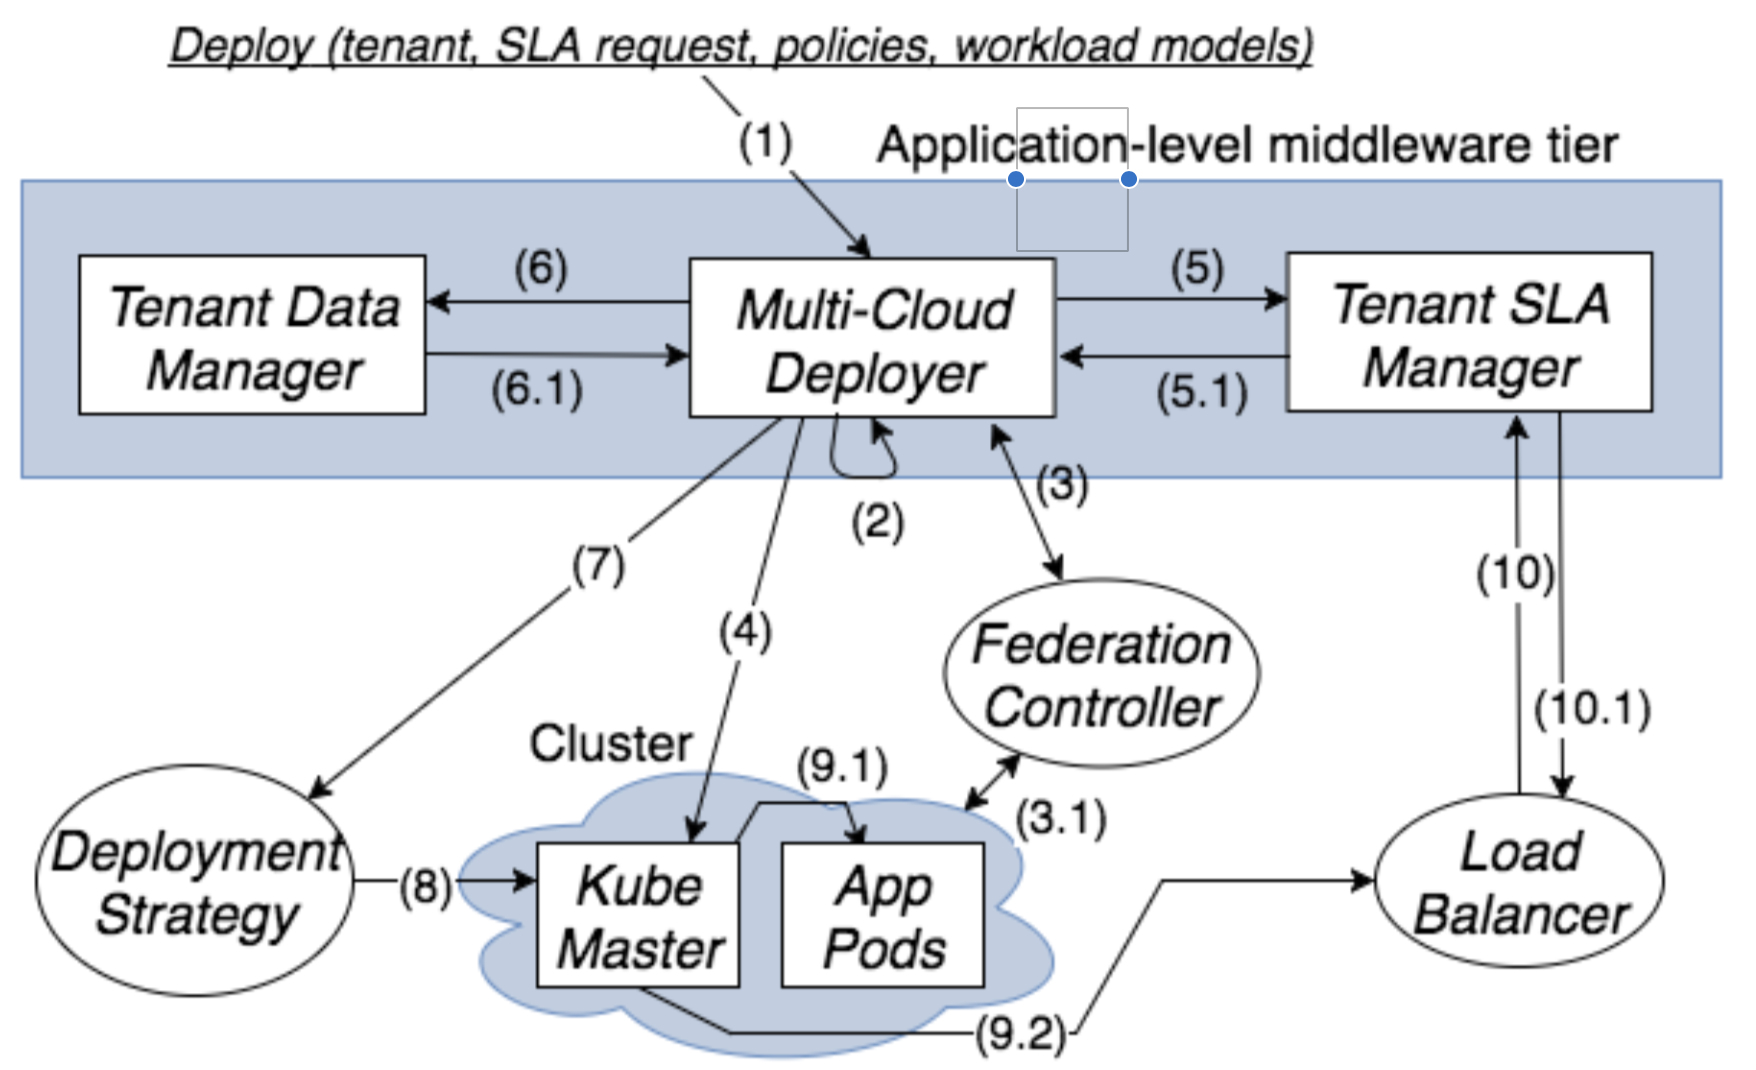
\includegraphics[width=0.6\textwidth]{chapter-related-work/images-eddy/middleware-eddy.png}
    \caption{Middleware architecture for multi-tenant SaaS applications.~\cite{TruyenEddy2016Taca}}
    \label{fig:eddy-architecture}
\end{figure}
\subsubsection{Architecture of middleware}
A possible high-level architecture presented by the paper is shown in Figure~\ref{fig:eddy-architecture}. It is composed out of three services, each implementing a policy-based architecture that can be extended with a control loop in which decisions are made based on application-centric monitoring.~\cite{TruyenEddy2016Taca}\\\\
The \textit{Multi-Cloud Deployer} is responsible for deploying SaaS application across multiple container orchestration clusters from different cloud providers. In this specific example architecture, it interacts with a Kubernetes cluster. It deploys namespaces and applications based on specifications delivered by the \textit{Tenant SLA Manager} and \textit{Tenant Data Manager}.~\cite{TruyenEddy2016Taca}\\\\
The \textit{Tenant SLA Manager} manages tenant SLAs and provides performance isolation by specifying the employed \textit{Requests and Limits} of the application containers in each namespace. It also manages admission control for each tenant via the front-end loadbalancer (assumed present for each application).
Lastly, the \textit{Tenant Data Manager} provides adaptive management of multiple database technologies.~\cite{TruyenEddy2016Taca}
\subsubsection{Deployment strategies}
The paper~\cite{TruyenEddy2016Taca} describes three possible deployment strategies for SaaS applications which employ container or container orchestration concepts. These strategies differ in the chosen trade-off between cost-efficiency and security isolation.

\paragraph{Shared container}
Each application instance of an existing multi-tenant application is allocated one container which is part of one pod. Each pod is run on a separate node. Resulting in each node in the cluster running one single container capable of handling client requests. The application instance must handle multi-tenancy itself (i.e., performance isolation and enabling tenant-specific features for all classes of tenants are handled at run-time). This approach shares resources at the highest level and does not leverage any security or performance isolation capabilities of the underlying container orchestration platform.\\\\
In terms of a Kubernetes specific deployment, clients connect to a single service (with a stable IP) which distribute requests among the pods. The pods are controlled by a single specified deployment configuration (next-generation replica controller).~\cite{TruyenEddy2016Taca}
\paragraph{Namespace per tenant}
Each tenant is assigned to its own separate, dedicated namespace. This allows to specify the exact resource requests and limits of pods needed to satisfy the SLA requirements of the tenant. Furthermore, it allows the container images to be tailored to solely load the tenant-specific features. In contrast to the previous strategy, here the advantages of the underlying platform such as security isolation between tenants are being used. However, this approach of using container orchestration as  middleware for multi-tenancy is less cost-efficient than the previous.\\\\
This strategy relies on the Kubernetes namespace concepts, allowing the division of cluster resources based on quota. For each namespace, a service and deployment have to be specified.  Tenant forward request to their corresponding services.~\cite{TruyenEddy2016Taca}
\paragraph{Namespace per SLA class}
The last proposed deployment strategy combines the previous two. Here tenants are grouped in distinguishing SLA classes. A separate, dedicated namespace with the corresponding quota is created for each class. The advantages of the previous approaches remain present to some extent. Sharing a container among tenants of the same class allows for a feature specific container and higher resource utilization but requires application-level admission control. It also allows for security between SLA-classes but not between tenants.~\cite{TruyenEddy2016Taca} 
\subsection{Conclusion multi-tenancy on K8 }
The previous section discussed proposals showing Kubernetes applicability for hard multi-tenancy achieving Containers as a Service (CaaS) or as an underlying platform for multi-tenant SaaS applications. In both scenarios, a trade-off is to be made between security isolation and cost-efficiency. Despite this, the proposals aim to maximize cost-efficiency while minimizing the complexity of cluster management or the complexity of additionally needed admission control. Kubernetes and container orchestration in general has the potential to be a building block for multi-tenant scenarios.

\subsection{Consequences of tenant aggregation}

\begin{figure}[H]
    \centering
    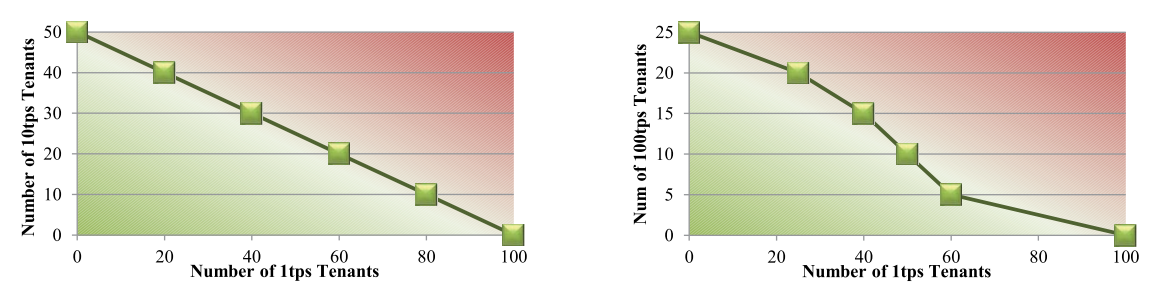
\includegraphics[width=0.9\textwidth]{chapter-related-work/images-towards-slos/sla-mix.png}
    \caption{Mix of different SLOs scheduled at a single SKU. Points above the frontier line represent scheduling policies failing to meet tenant SLOs. Point on the frontier line meet all tenant SLOs. Scheduling policies in the area below the frontier line satisfy tenant SLOs but potentially waste resources.~\cite{lang2014towards}}
    \label{fig:sla-mix}
\end{figure}
The work of~\cite{lang2014towards} specifies the challenges of balancing multi-tenancy performance and operation costs in the context of performance-based Service-Level-Objectives SLOs for a Database-as-a-Service (DaaS) provider. The challenge is the specification of a hardware provisioning policy and a tenant scheduling. The former refers to the selection of machines (possibly different SKUs) needed for a given set of tenants. The latter is the mapping between tenants and provisioned SKUs that minimizes costs while meeting the SLO's performance goals. Figure~\ref{fig:sla-mix} shows the alteration between homogeneous and heterogeneous tenant mixes of two SLOs on a single SKU. The frontier line shows the mix of tenant SLOs that satisfy all tenant SLOs without the waste of resources. When the frontier is linear (left), a provider can easily define a scheduling policy. However this is not always the case, as different parts of the system can become a bottleneck. The allocation problem becomes even more complex with a mix of SKUs.~\cite{lang2014towards} \\\\
The authors propose a three-step plan for tackling this problem. Starting by determining the upper boundary for homogeneous tenants mixes of every SLO $s_{i}$ on all available SKUs (i.e., how many tenants of class $s_{i}$ can be scheduled on SKU without violating the SLOs). Secondly, a characterization function $\hat{f}(\vec{b})$ for each SKU is evaluated where $b_{i}$ is the number of tenants of class $s_{i}$. The function returns either the average performance for each tenant class or $false$. A systematic search is employed to determine solely the values for which  $\hat{f}$ is true, essentially constructing the frontier. The search starts from a homogeneous mix of high-performance tenants (output step 1) and iterative substituting a fixed small number of highest-performance tenants with low-performance tenants until SLOs are violated. When dealing with more than two SLOs all combinations need to be benchmarked. Using the characterization functions from the first two steps an optimization problem is formulated. A brute-force solver is used that explores the feasible regions.~\cite{lang2014towards}

\section{Dealing with Service Level Objectives}

\subsection{Morpheus: Towards automated SLOs for enterprise clusters}
\label{rw:morpheus}
Morpheus~\cite{jyothi2016morpheus} is a state-of-art cluster scheduler for recurring batch jobs. It presents interesting features such as the programmatic derivation of SLOs and job resources enabling a \textit{tuning-free} experience for its users. Starting from a user study showing that users of a shared cluster are 120x more likely to complain about the (un)predictable completion time of their job than about the fairness of sharing. The study results also showed a wide range of under/over-allocation of job resources confirming the difficulty of manual tuning. The data-driven solution, briefly discussed below, is optimized for end-user satisfaction while being able to reduce the required cluster footprint.
\begin{figure}[H]
    \centering
    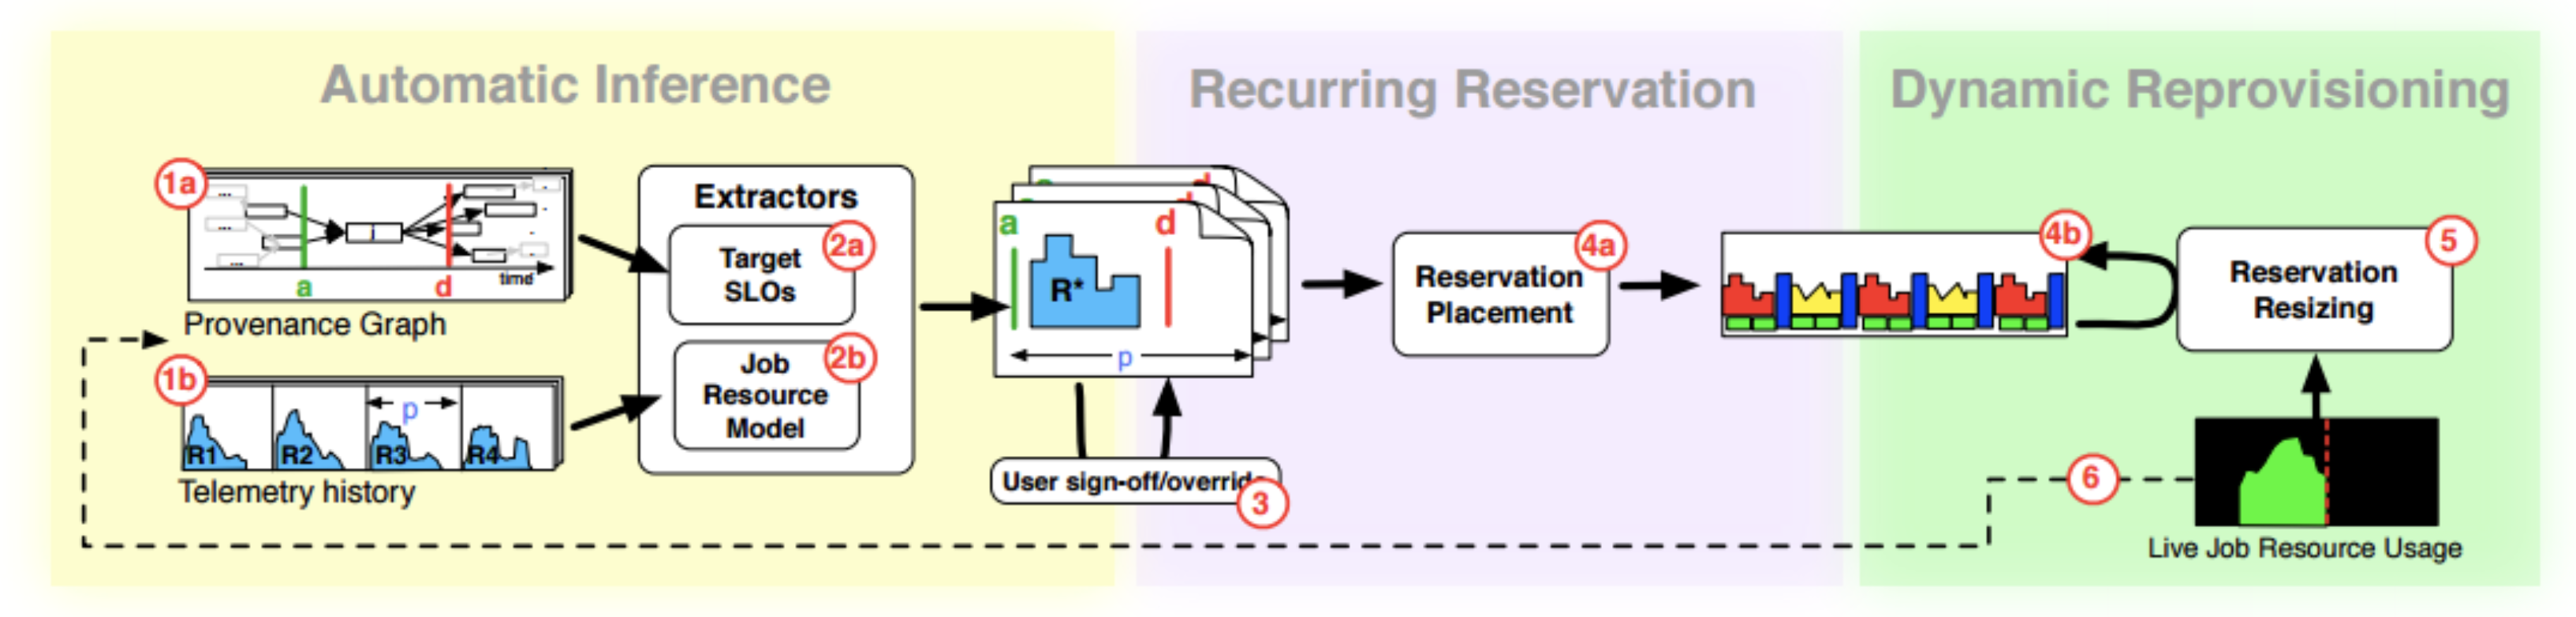
\includegraphics[width=0.9\textwidth]{chapter-related-work/images-morpheus/morpheus-fig.png}
    \caption{Life-cycle of a recurring job in Morpheus.~\cite{jyothi2016morpheus}.}
    \label{fig:morpheus}
\end{figure}
\paragraph{Extraction of target SLOs}
 SLOs in Morpheus are focused on job completion by deadline, the one observable metric its users care about. The extractor, responsible for the derivation of these deadlines, utilizes a provenance graph (PG). The PG is a graph representation of key properties of job and system information built from application, file-system and front-end logs. Individual jobs are grouped into periodic jobs by means of templating (based on job names, code signatures and inter-arrival times). By the use of statistics on the history of grouped jobs, a deadline can be offered.
\paragraph{Extraction of job resources}
For the inference of job resources, the extractor relies on the input of detailed telemetry information. Based on time-series of resource utilization from multiple job runs, Morpheus solves a linear programming optimization problem (including terms for over- and under-allocation penalties) to find the best fit for all historic patterns. It thus produces a resource allocation that approximates the actual requirements of the periodic job.~\cite{jyothi2016morpheus}
\paragraph{User sign-off or override}
The inferred SLO and resource model is presented to the user in the form of a recurring reservation request. He/she has the ability to either sign of on the proposal, add further knowledge to the proposal by overriding parameters or reject the proposal. In the last case the job is executed using the standard fair-queuing semantics of the cluster.~\cite{jyothi2016morpheus}
\paragraph{Reservation placement}
Upon approval, the recurring reservation request is a reservation placement mechanism. Morpheus extends YARN's standard reservation system with a novel online packing algorithm specialized for periodic jobs, called LowCost. For the details, the consultation of the paper is recommended. The use of reservations enables to prevent unpredictability introduced by a shared environment. Recurring jobs are scheduled in a manner that isolates them from each others noise (e.g., non-interfering workloads, which do  stress the same resource type, will not be allocated on the same node).~\cite{jyothi2016morpheus}
\paragraph{Dynamic reprovisioning}
While LowCost eliminates sharing-induced unpredictability, Morpheus has to deal with the challenge of inherent unpredictability. Examples of factors that introduce performance variance include but are not limited to, changes in SKUs (different machine configurations - Stock Keeping Units), code base changes or skew in input data. These issues are mitigated by a dynamic re-provisioning algorithm which continuously monitors a job's resource consumption. For a slower-than-expected job, the resources are enlarged. The resource consumption is constantly fed back to back to the provenance graph and telemetry information for future job runs.~\cite{jyothi2016morpheus}

\subsection{SLA Decomposition: Translating Service Level Objectives to System Level Thresholds}
In SLA Decomposition~\cite{chen2007sla} Yuan Chen \textit{et al.} present an approach for translating SLOs to lower-level resource quotas for each component of a web service. Their solution combines \textit{performance modeling} with \textit{performance profiling} to create models. Traditionally, these complex translations are made by domain-experts relying on past experience with specific applications deployed in a particular environment. Design decisions about operating systems, middleware, infrastructure and the inherent dynamism of systems make the automated derivation of system thresholds from high-level goals (SLAs) a difficult challenge.~\cite{chen2007sla}\\
The definition of the SLA-decomposition and approach from the paper are  discussed in this section.
\subsubsection{SLA decomposition task}
In the paper, the SLA decomposition task is defined as finding a mapping between  service level objectives (e.g., response time and throughput) and the state of each individual component in the system (e.g., resource requirements and configuration). An example from the paper is given the SLOs $(R,T)$, expressing objects on \textit{Request latency} and \textit{Request throughput}, and a typical 3-tier application composed out of n HTTP server, an application server and a database, the decomposition is finding the following mapping:
\begin{equation}
(R,T) \rightarrow (\theta_{http-cpu},\theta_{http-mem},\theta_{app-cpu},\theta_{app-mem},\theta_{db-cpu},\theta_{db-mem} )
\end{equation}
The problem of SLA decomposition can be viewed as the inverse of the performance modeling. In performance modeling, a model based on resource utilization and configuration settings is used to predict the overall system's performance.~\cite{chen2007sla}


\subsubsection{SLA decomposition approach}
\begin{figure}[H]
    \centering
    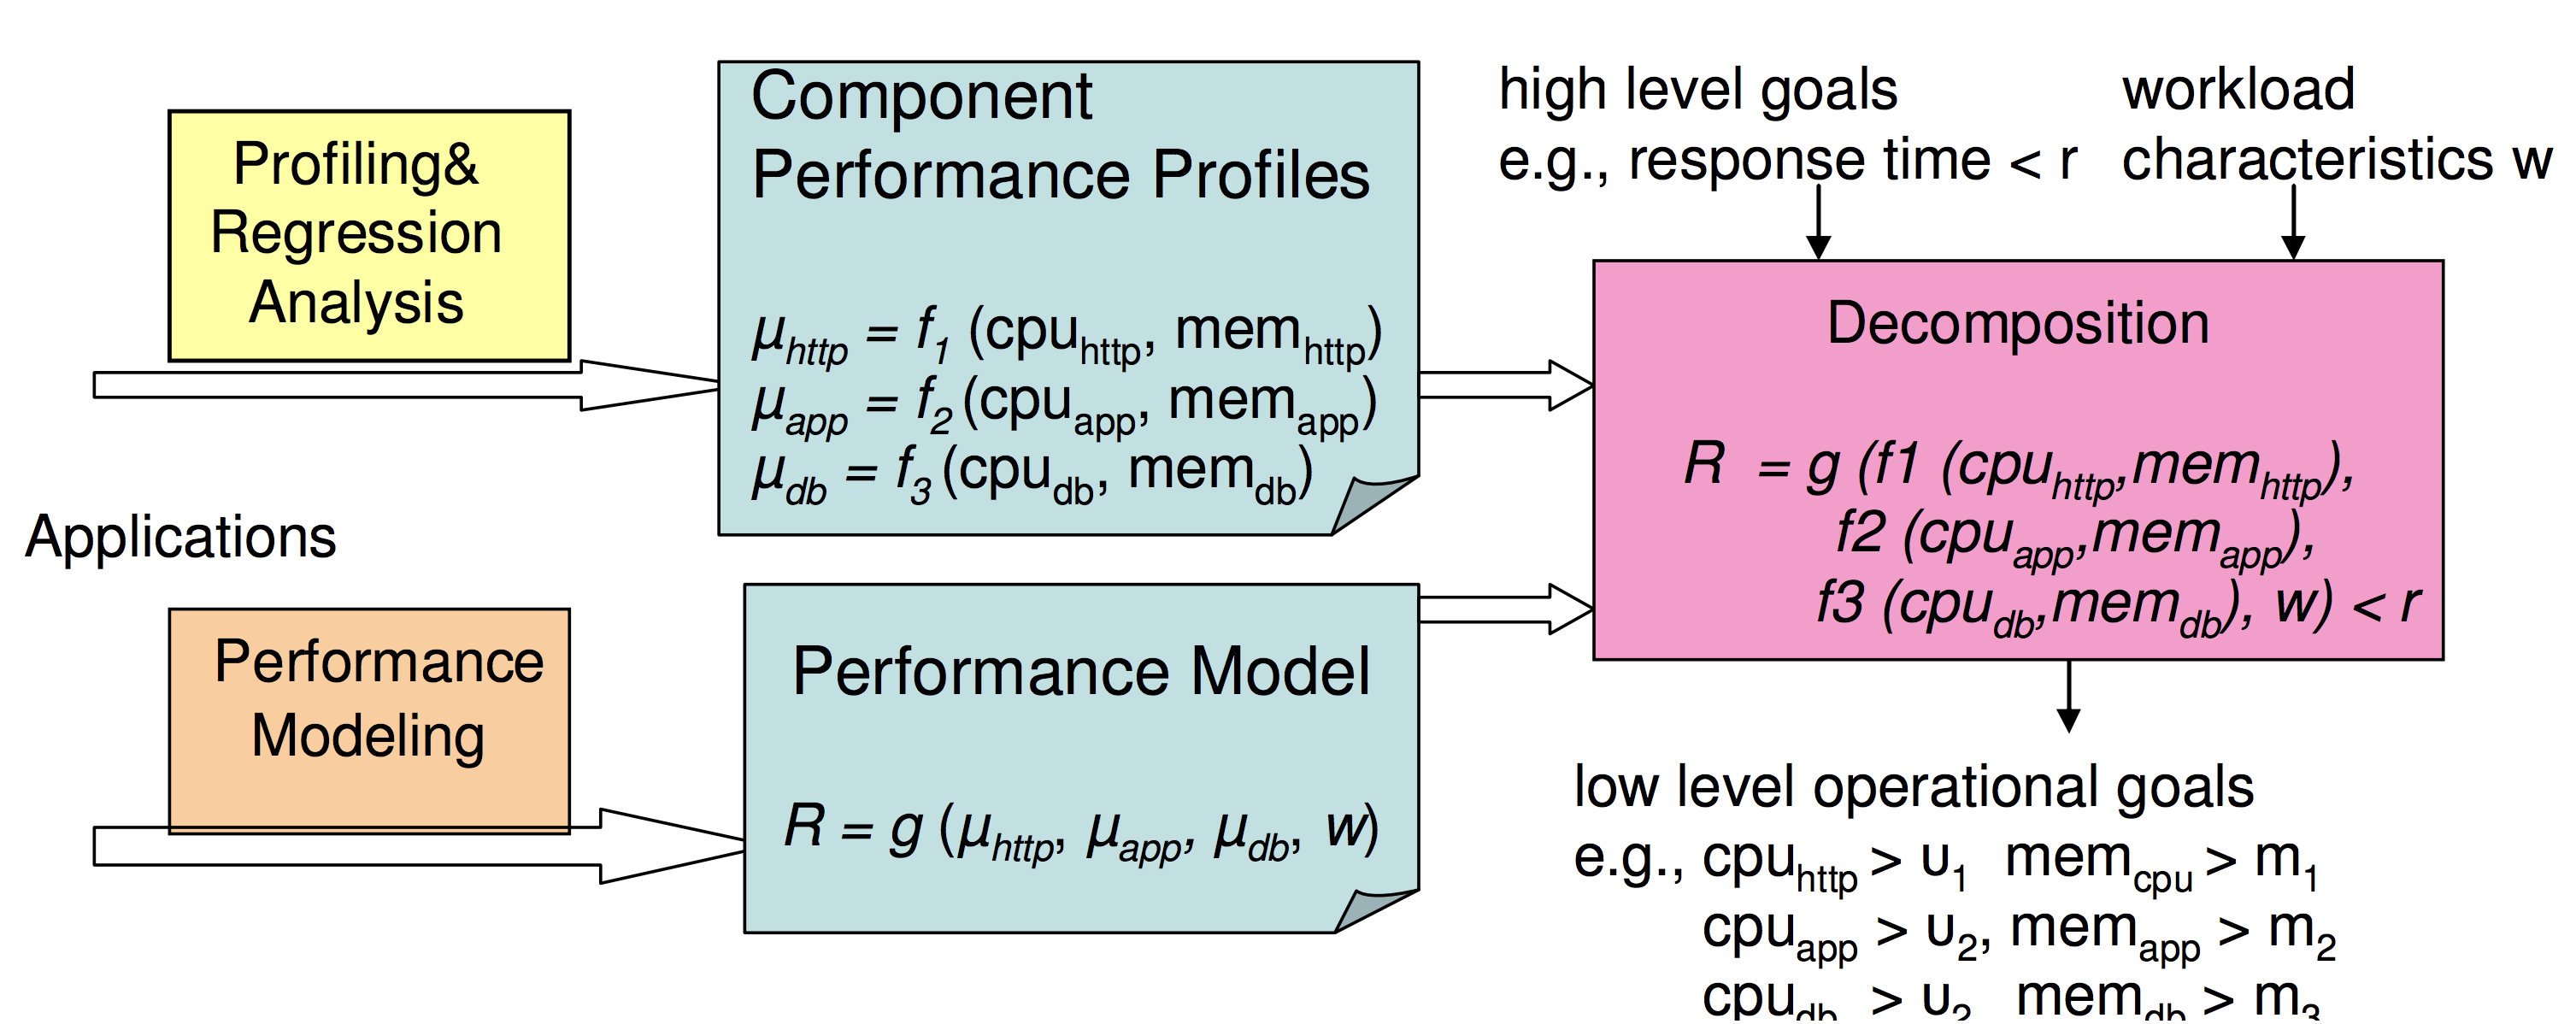
\includegraphics[width=0.7\textwidth]{chapter-related-work/images-decomp/sla-decomp-paper.png}
    \caption{Conceptual architecture of approach for SLA decomposition by~\cite{chen2007sla}.}
    \label{fig:decomp-architecture}
\end{figure}

Figure~\ref{fig:decomp-architecture} illustrates the presented approach of~\cite{chen2007sla} to tackle the SLA decomposition problem. It builds components performance profiles and a performance  model and combines them to solve the decomposition problem. Each step is briefly explained below. \\\\
\textbf{Component profiling:} A component profile characterizes a component's performance as a function of resource allocation (e.g., memory, CPU) and configuration. This function is derived using a regression-based approach on performance measurements of the component such as mean service rate $\mu$. The measurements are obtained from benchmarks with a variety of workloads in which resource allocations of the component are altered in each iteration. The result of this step is a function of the following form for each component:
\begin{equation}
 \mu = f(CPU,MEM)
\end{equation}
\noindent\textbf{Performance modeling:} A performance model is used to define the relation between every single component and the overall system performance. Given a particular workload $w$ and set of components' performance characteristics, the model predicts the performance of the combined components. For the 3-tiered web service the model $g$ for response time is proposed :
\begin{equation}
 R = g(f_{http}(CPU,MEM),f_{app}(CPU,MEM),f_{db}(CPU,MEM), w)
\end{equation}
To obtain such a model, the paper proposes to model the multi-tier web service as a novel queuing network model. Each tier is represented in the network as a multi-station queuing center (i.e., G/G/K queue), illustrated in Figure~\ref{fig:decomp-muti-queue}. This reflects the commonly used  multi-threaded architecture of servers. The performance of the queuing network is evaluated using Mean-value analysis (MVA). Using this approach, the authors claim that the performance of a multi-tier application can be accurately predicted using single tier's performance and workload characteristics.  The details of the model and analysis are omitted in this thesis.~\cite{chen2007sla}

\begin{figure}[H]
    \centering
    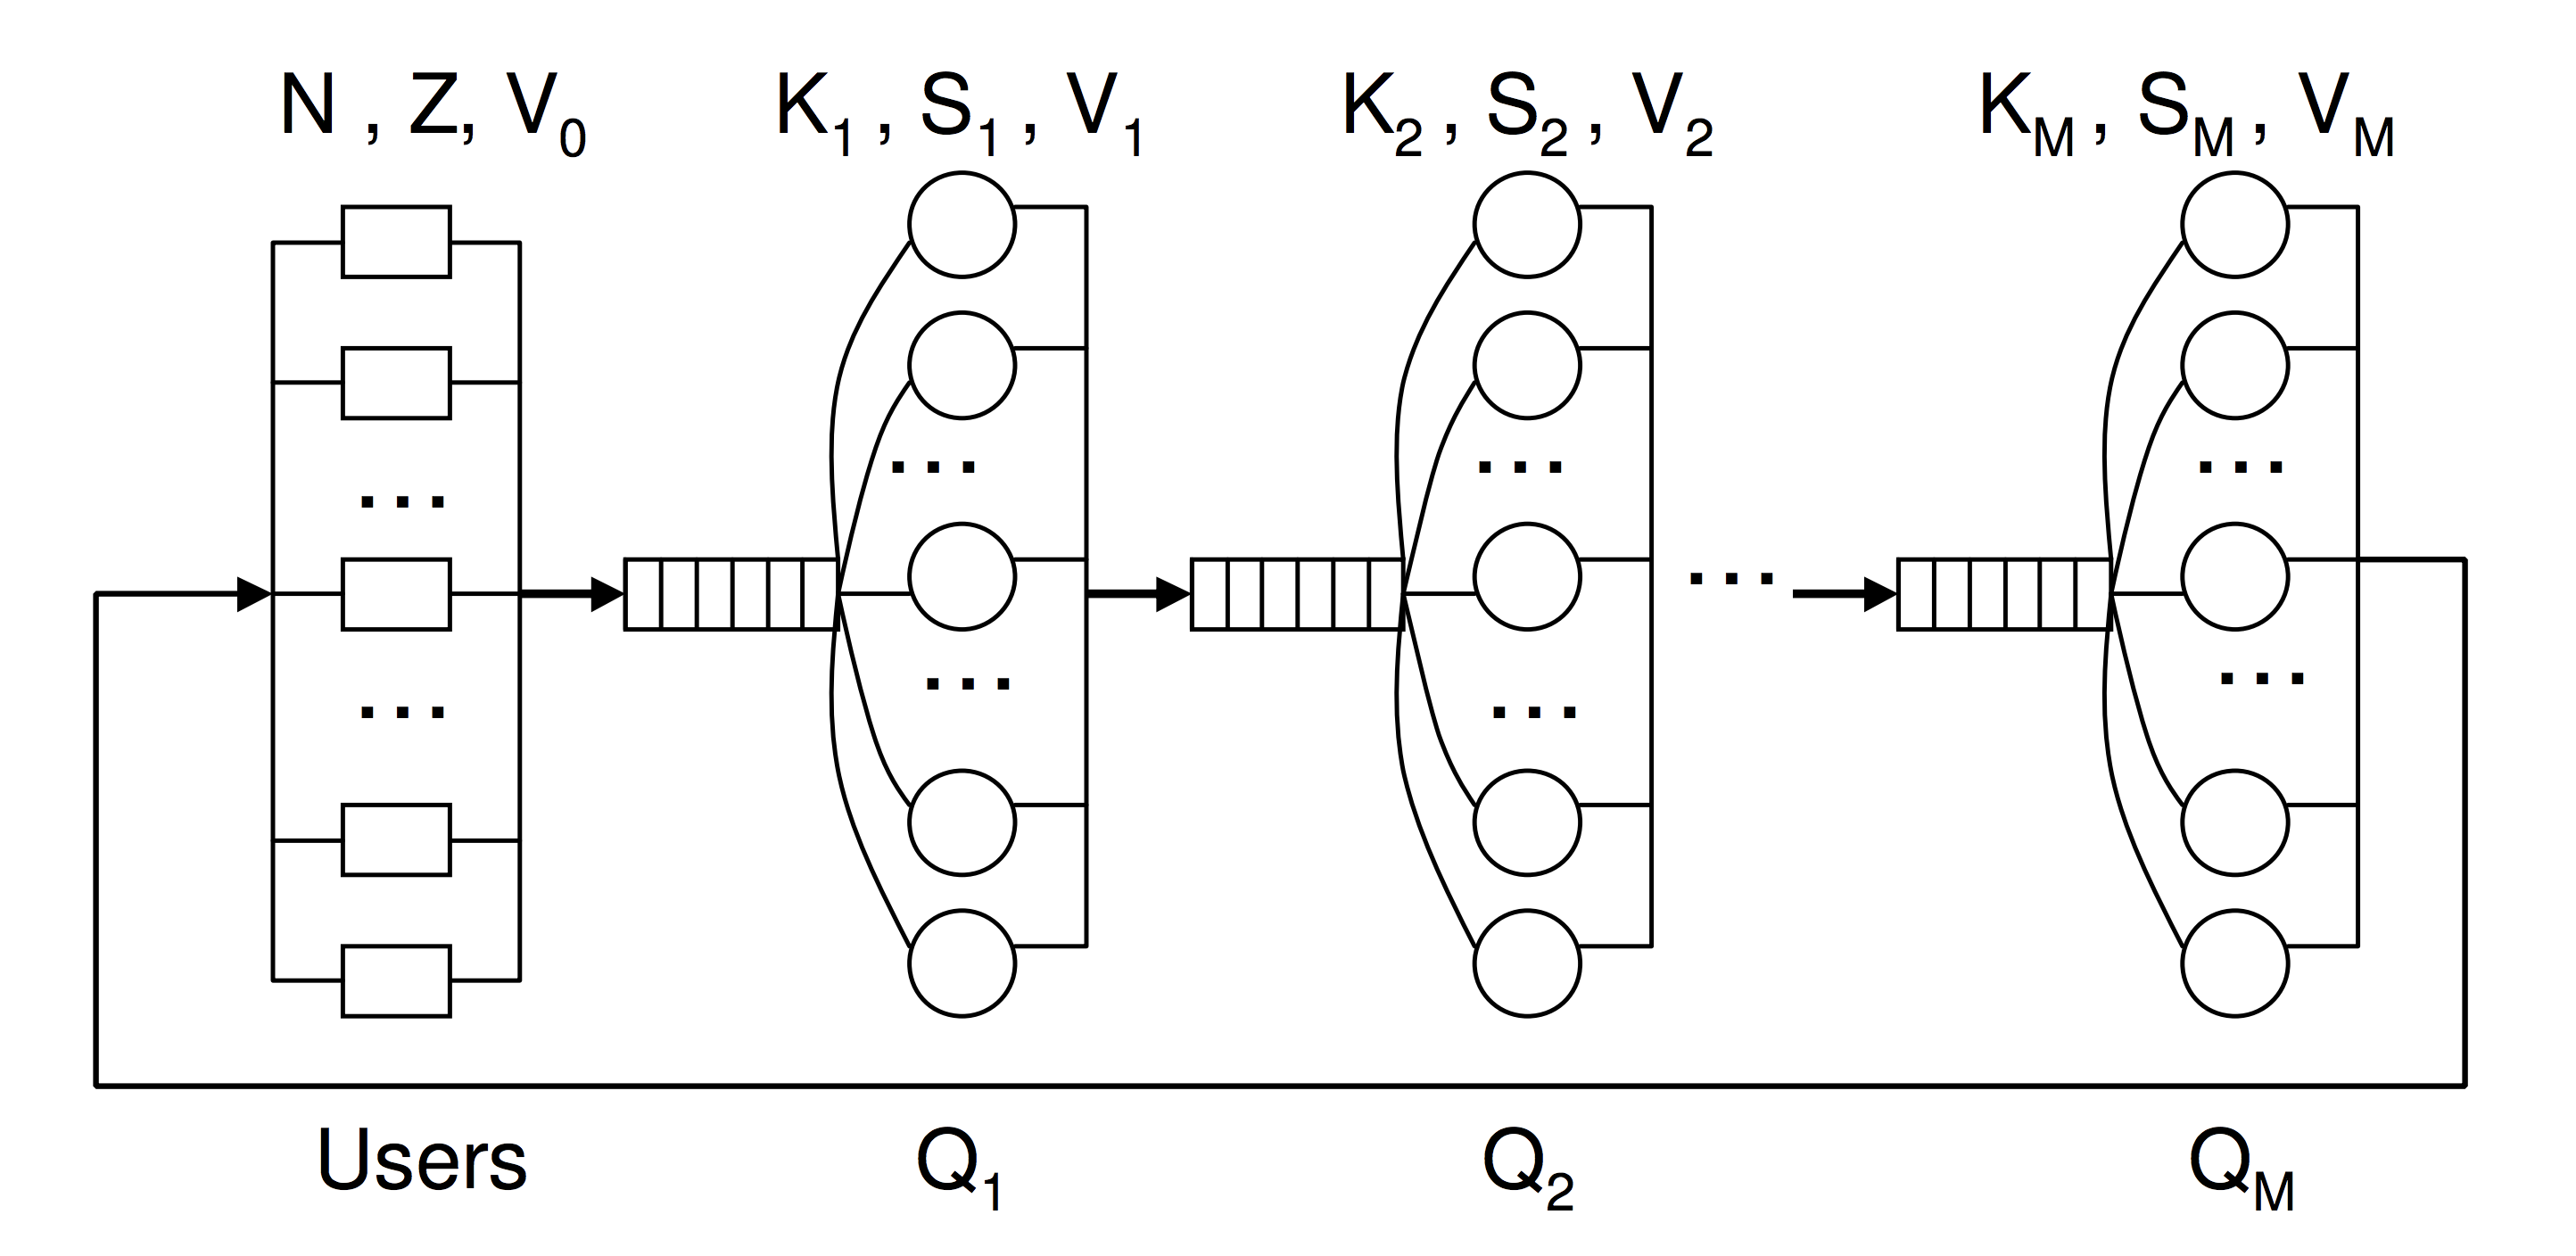
\includegraphics[width=0.6\textwidth]{chapter-related-work/images-decomp/sla-decomp-multi-queue.png}
    \caption{Multi-tier web application represented as a closed multi-station queuing network. It models $N$ concurrent users sessions. A user session consists of a succession of requests with a think time $Z$  between each request. Each tier $i$ is represented by queue $Q_{i}$ with $K_{i}$ worker threads. $S_{i}$ and $V_{i}$ respectively represent the mean service rate and mean request rate of tier $i$. $V_{0}$ denotes the average request rate issued by the users.~\cite{chen2007sla}}
    \label{fig:decomp-muti-queue}
\end{figure}

\noindent\textbf{Decomposition:}
Given both performance profiles and performance models for performance characteristics used in the SLOs, using the corresponding equations the decomposition problem can be defined as a constraint satisfaction problem. An example of such a problem with constraints maximum response time $r$ and minimum throughput $X$ is given below:
\begin{align*}
g(f_{http}(CPU_{http}),f_{app}(CPU_{http}),f_{db}(CPU_{db}), w) < r \\ g(f_{http}(CPU_{http}),f_{app}(CPU_{http}),f_{db}(CPU_{db}), w ) > x 
\end{align*}
For solving constraint problems various methods exist such as linear programming or optimization techniques. However, the solution space is often large and the solution is non-deterministic. As a remedy, the authors suggest the employment of a coarser granularity of parameters (e.g., 5\% CPU slices) to minimize the search space or the use of heuristics (e.g., response time minimizes with an increase of CPU) for a more efficient search. The search may halt as soon as a feasible solution is found.~\cite{chen2007sla} \\\\
In~\cite{barna2017delivering}, a similar approach is used. A three-layered queuing network of resources is used as a performance model for containerized cloud applications. The layers respectively correspond to applications, containers and virtual machines. In contrast to component profiling, the paper implements Kalman filters~\cite{kalman1960new} in a MAPE-K~\cite{de2013software} based architecture in order to estimate the model parameters. Values gathered by the \textit{Monitoring} and \textit{Analysis} modules are evaluated towards specific thresholds (depending on the service level objectives). The \textit{planning} module uses the performance model to determine resource scaling actions based upon the violation of one of the thresholds. In order to deal with the irregularities of web traffic, a \textit{Scaling Heat algorithm} is proposed to avoid unnecessary scaling actions.


\subsection{Automated configuration tuning: Best Config}
\label{rw:bestconfig}
The paper \textit{BestConfig: Tapping the Performance Potential of Systems via Automatic configuration tuning}~\cite{zhu2017bestconfig}  presents an automatic configuration tuning system for general systems in the cloud that can optimize performance goals by adjusting configuration parameters. It recommends the best configuration found within a limit number of allowed tests. This is achieved by combining an effective sampling method called \textit{divide-and-diverge sampling} and \textit{recursive-bound-and-search}, a search-based optimization algorithm. Both are  discussed in the remainder of this section.
\subsubsection{Parameter tuning}
A good configuration setting can lead to a strong improvement of a system's performance, especially for systems with a recurring workload. Performance tuning refers to the process of searching for the configuration with the best performance. In a manual setting, the process consists of finding a heuristic approximating the performance model of the system, adjusting configuration setting based on the model, running benchmarks and observing the corresponding performance. If the desired performance is not achieved, the heuristics need to be adjusted and the process is repeated. Resulting in a time-consuming and labors process. In addition, the growing number of configuration parameters  of recent systems (e.g., 180 in Hadoop) can lead to complex configuration issues and complicates the search for heuristics.~\cite{zhu2017bestconfig}\\\\
\noindent BestConfig tries to address the challenges of automatic configuration tuning simultaneously. By offering a decoupled architecture, it is possible to \textit{support a variety of systems, workloads and deployment environments}. Easy usage within the deployment environment, is necessary because the deployment environment can  heavily influence a system's performance model. Furthermore, the high number of parameters in recent systems led to a \textit{high-dimensional parameter space}. The high cost of sampling makes it impossible to get a complete image of the mapping between all configurations and their performance. Since building a performance simulator (e.g., Starfish~\cite{herodotou2011starfish} for Hadoop) for every system is unfeasible, automatic configuration tuning should work with a \textit{limited amount of samples}. In addition,  it should allow the result to be improved when the number of samples increases. Lastly, performance is represented in different metrics for different systems. For example, for a data analytic cluster  the goal might be to reduce the total run time, while for a web service the throughput needs to be maximized. Some systems might even have multiple performance goals.~\cite{zhu2017bestconfig}
\subsubsection{Divide \& diverge sampling (DDS)}
In order to get a wide coverage of the high-dimensional parameter space, in BestConfig it is \textit{divided} into subspaces. Given $n$ parameters, each parameter's range is divided into $k$ intervals. Combining a sample from each interval results in a sample set with a  granularity exponential to the number of parameter dimensions (i.e., $k^n$ combinations). This is illustrated in Figure~\ref{fig:bestconfig-DDS} by all the dots. Resulting in a high cost for sampling. The authors suggest, to reduce the granularity but keep a wide coverage,  the sample set can be \textit{diverged} the most by representing each interval of each parameter exactly once. They observed that the combination of all parameter intervals is nonessential since: \textit{"the impact of an influential parameter's value on the performance can be demonstrated through the comparisons of performances, disregard of other parameters' value~\cite{zhu2017bestconfig}"}. In  Figure~\ref{fig:bestconfig-DDS}, the green dots are thus the selected samples to be tested. With a larger resource limit (i.e., number of tests), the number of intervals $k$ can be increased, resulting in a better image of the parameters space. Resulting in a scalable sampling method.~\cite{zhu2017bestconfig}
\begin{figure}
\centering
\subfigure[Illustration of BestConfig's DDS on a 2D parameter space. Dots represent all combination of sampled parameter spaces. Blue lines indicate sampling intervals. Green dots are the selected dots after random divergence.]{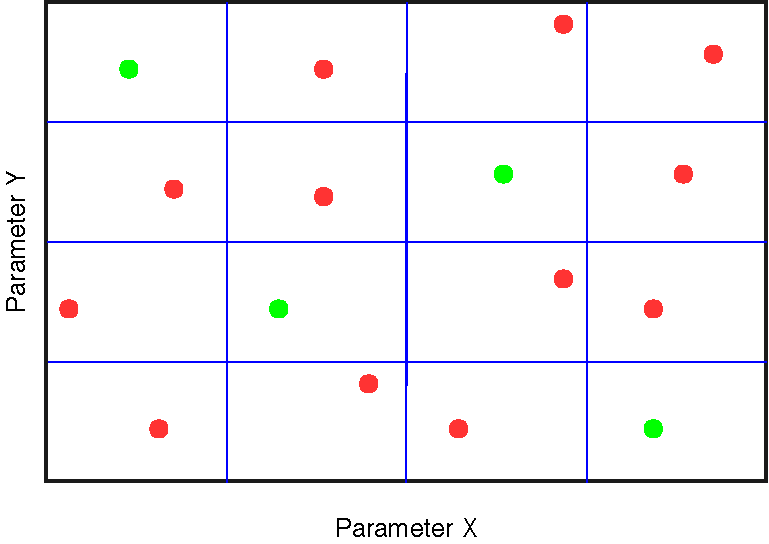
\includegraphics[width=0.7\linewidth]{chapter-related-work/images-bestconfig/bestconfig_divide_diverge_sampling.pdf}\label{fig:bestconfig-DDS}}
\subfigure[Illustration of BestConfig's RBS on a 2D parameter space. The blue dot $C_0$ indicates the parameter combination with the highest score on the utility function. The bounded space represents the search space for the next iteration.]{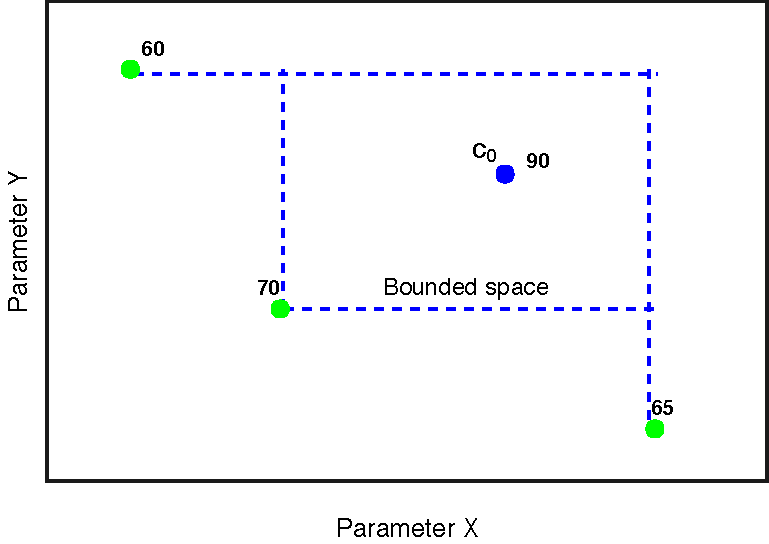
\includegraphics[width=0.7\linewidth]{chapter-related-work/images-bestconfig/bestconfig_RBS.pdf}\label{fig:bestconfig-RBS}}

\caption{Illustration of BestConfig's DDS \&  RBS.}
\end{figure}


\subsubsection{Utility function}
For simplicity, RBS (explained in the next paragraph) optimizes towards a single, scalar performance metric. This metric is retrieved from a \textit{utility function} which has user-concerned performance goals as inputs. In other words, it translates the  benchmark result of a sample configuration into a single score. This score is either minimized or maximized by BestConfig. This function is defined by the user.  An example given in the paper of a utility function $f$, where a user wants to increase throughput $x$ and decrease latency $l$ is:
\begin{equation}
    f(x_{t},x_{l}) = \frac{x_{t}}{x_{l}}
\end{equation}

\begin{figure}
    \centering
    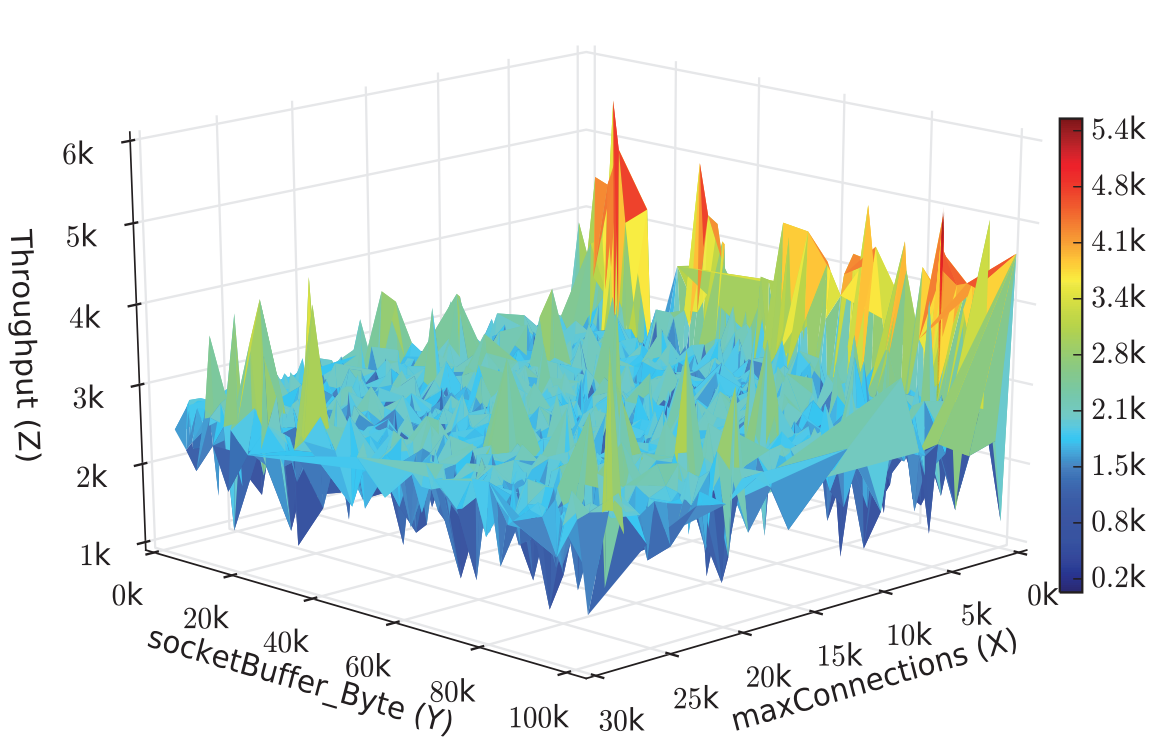
\includegraphics[width=0.6\textwidth]{chapter-related-work/images-bestconfig/bestconfig-surface.png}
    \caption{The performance surface of a tomcat server. The employed utility function reflects the throughput of a sample configuration.~\cite{zhu2017bestconfig} }
    \label{fig:bestconfig-surface}
\end{figure}


\subsubsection{Recursive Bound \& search (RBS)}
Figure~\ref{fig:bestconfig-surface} shows the complete performance surface of a tomcat server. It shows the performance metric presented by the utility function, namely throughput. The goal of a performance optimization algorithm (PO) is to find the best configuration with a limited view of the performance surface. This view is the result of benchmarks on the sample set chosen by DDS. RBS is a search-based PO that builds on the following assumption of continuous  performance surfaces: \textit{Given a continuous surface, there is a high possibility of finding other points with similar or better performance around the point with the best performance in the sample set~\cite{zhu2017bestconfig}.} RBS thus searches the area near the sample $C_{0}$ awarded the highest score by the utility function. This area is referred to as the \textit{bounded space}. The bounds of this space are chosen in the following manner for each parameter $p_{i}$. The new lower-bound for a parameter $p_{i}^{min}$ is the largest value of $p_{i}$ in the sample set that is smaller $p_{i}$ of sample $C_{0}$. The upper bound for a parameter $p_{i}^{max}$ is the smallest value $p_{i}$ in the sample set that is larger than $p_{i}$  of sample $C_{0}$. This is illustrated in Figure~\ref{fig:bestconfig-RBS}. If the resource limit (number of iterations) has not been exceeded, DDS is repeated with the new parameter ranges, as defined by the bounded space. Otherwise, $C_{0}$ is returned as the best found configuration.~\cite{zhu2017bestconfig}\\\\
However, the PO might get stuck in local sub-optimum and consequently possibly not find the global optimum, even when given sufficient resources. To mitigate this case, BestConfig added the possibility of a recursive step. If no sample with better performance is found in a new round, RBS simply restarts from the beginning with the complete parameter space. The paper gives a detailed explanation on why the combination of DDS and RBS works. This discussion is omitted in this thesis.~\cite{zhu2017bestconfig}
\subsubsection{Model-based method for performance tuning}
Besides search-based approaches, it is also possible to use a model-based performance optimization algorithm. The authors of BestConfig argue that these methods require a larger number of samples given a high-dimensional parameter space and rely heavily on the knowledge of the developer. For example, the developer needs to know if the model is quadratic or linear but with a large number of components in deployments predicting this has shown to be a difficult task. Lastly, models often require the configuration of hyper-parameters, which is a tuning problem itself. To prove the in-feasibility of model-based approaches, BestConfig was compared to both Co-training Model Tree (COMT)~\cite{chen2013effective} and Gaussian Process Regression (GPR)~\cite{duan2009tuning}. The results show that the models make bad assumptions about the system resulting in wrong predictions, cannot output a competitive configuration compared to BestConfig and tend to over-fit when given more resources.~\cite{zhu2017bestconfig}


% \subsection{Utility functions in autonomic systems}
% The employment of utility functions for the optimization guidance of systems is nothing new. In \cite{walsh2004utility} a two-level self-optimizing architecture based on utility functions is introduced for heterogeneous application environments. The higher level periodically recomputes the resource allocation (e.g, nodes) that maximizes a global utility function (i.e.,maximize the sum of user satisfaction for all application environments). This global function is defined in terms the resources utility functions $\hat{U}(\textbf{R})$ of all present application environments, determined at the lower level. At the lower level, separately for each application environment, a controller is responsible for the computation of the control parameters $C$. To achieve this, it optimizes the service level utility function $U(S,D)$ based on the application's performance model $S(C,R_{t},D)$ and with current resource level $R_{t}$ and current demand $D$. The service level utility expressed the users satisfaction for a given service $S$ at a current demand $D$. The resource utility function $\hat{U}(\textbf{R})$ is derived by calculation the optimal service level utility for all possible resource levels $R$ given the next predicted demand $D'$ of the application. The authors point out that the approach requires the specification of an accurate performance model \textit{a priori}, a demand forecaster and a solver for the NP-hard discrete resource allocation problem that is specified by the global utility function. \\
% The evaluation by the authors shows the applicability of the approach for node allocation in a cluster of web applications handling transaction workloads. \cite{costache2017resource} mentions several improvements \cite{nguyen2009autonomic} \cite{van2010performance} on this work by moving to allocation of VMs instead of nodes and the addition of provider objectives (e.g. minimize the number of employed nodes).

\subsection{Bayesian optimization as performance model for search minimization}
\label{rw:cherry}
Big data analytics face a similar configuration problem due to the rapid growth of available techniques and frameworks such as MapReduce, Spark and others. Finding a better configuration can result in large cost and time savings. CherryPick~\cite{alipourfard2017cherrypick} is an optimization tuner for various applications that exploits the characteristics of Bayesian optimization to obtain accurate enough performance models in order minimize the search for an optimal or nearly-optimal configuration. The authors point out similar restrictions of both poorly adaptive model-based and costly exhaustive search approaches as mentioned in  previous sections.\\\\
The use of Bayesian optimization allows to achieve several key characteristics wanted of an auto tuner. Adaptivity is possible since the approach treats every application as a black-box. The obtained models are solely accurate enough to rank configurations. By adapting the model every run, an interactive search can be conducted, resulting in low overhead.~\cite{alipourfard2017cherrypick} \\\\
A run of the interactive search consists of running a job with a configuration, building and updating a black box model (relation between settings and cost/performance constraints), ranking configurations based on model and choosing the next configuration to run. The steps are repeated until the accuracy is high enough. Bayesian optimization has two components: a prior function and an acquisition function. The former models the cost and performance of the jobs by giving a confidence interval of possible fitting functions. The later is used for ranking the (remaining) configurations, it calculates the expected improvement compared to the current best configuration. This allows to emit areas in the space search with less promising configurations. An additional advantage of Bayesian optimization is its capability to incorporate additive noise into the confidence interval. This noise can be observed from historical data. A naive solution would be to run tests multiple times, resulting in a larger overhead.~\cite{alipourfard2017cherrypick} 
 
\section{Conclusion}
\label{rw:conclusion}
The related work discussed in the first section of this chapter shows that search for approaches to achieve multi-tenancy on top of container orchestration, specifically Kubernetes, is an active and interesting research topic. The fine-grained control of compute resources and flexible deployment offered by container orchestration can potentially be leveraged by SaaS providers to maximize their cost-efficiency while respecting their customer's SLAs. However, finding the best configuration for each application has proven to be a difficult task for developers and system administrators in general.\\\\
Approaches, discussed in this chapter, to deal with the assignment of resource thresholds in the presence of SLAs can be distinguished by whether or not performance models are used to search the best possible configuration. Model-based approaches suffer from several drawbacks such as high complexity for administrators, poorly adaptive to different applications and the requirement of extensive knowledge on the inner workings of an application. In addition, models do not guarantee the requirement of fewer configuration tests and even tend to overfit when offered more samples.\\\\
The optimization approaches mentioned in Sections \ref{rw:bestconfig} and \ref{rw:cherry} treat the application as a black box and do not require the construction of a model of the application. The use of general optimization techniques offers better adaptivity to a variety of applications. In terms of usability, BestConfig's utility function is slightly more intuitive than CherryPick's Bayesian optimization. BestConfig's evaluation of configurations through continuous experimentation, eliminates uncertainty on the quality of the results present in predictions by model-based approaches.  Therefore BestConfig's performance optimization algorithm is selected as the basis of the SLA-decomposition approach presented in this thesis. In the next chapter, it is adapted to fit the SLA-decomposition problem and implemented as part of a proof-of-concept.